\documentclass[12pt, a4paper]{article}

\usepackage[utf8]{inputenc}
\usepackage[T1]{fontenc}
\usepackage[russian]{babel}
\usepackage[oglav,spisok,boldsect, figwhole]{./style/fn2kursstyle1}
\graphicspath{{./style/}{./figures/}}
%\usepackage{float}%"Плавающие" картинки
\usepackage{multirow}
\usepackage{subcaption}
%Римские цифры
\newcommand{\RomanNumeralCaps}[1]
{\MakeUppercase{\romannumeral #1}}

\usepackage{comment}

%Параметры титульника
\title{Прямые методы решения СЛАУ}
\group{ФН2-52Б}
\author{Г.А.~Швецов}
\supervisor{С.А.~Конев}
\date{2022}
\begin{document}
	\newcommand{\pl}{\partial}
	\maketitle
	
	\tableofcontents
	
	\newpage
	\section{Общие сведения о прямых методах решения СЛАУ}
	\textbf{Прямыми} называют методы решения СЛАУ, которые позволяют получить точное решение за конечное число действий при
	условии, что все арифметические действия выполняются точно (без погрешностей).
	В данной лабораторной работе рассмотрим два прямых метода:
	метод Гаусса и метод QR-разложения.
	\section{Метод Гаусса (с полным или частичным выбором главного элемента)}
	\subsection{Метод Гаусса}
	Метод Гаусса заключается в последовательном исключении неизвестных $x_j,\\j=1,2,\dots,n-1,$ из системы:
	\[
	\sum_{j=1}^n a_{ij}x_j=b_j,\;	
	i=1,2,\dots,n.		
	\]
	В результате она преобразуется, пересчитав коэффициенты $a_{ij}^{(k)}$ и $b_i^{(k)}$, к эквивалентной системе с треугольной матрицей. Такой процесс называется \textbf{прямым ходом метода Гаусса.}
	Затем неизвестные $x_i$ последовательно, начиная с $x_n$, определяются по формулам:
	\[
	x_i=\left(b_i^{(i-1)}-\sum_{j=i+1}^n a_{ij}^{(i-1)}x_j\right)/a_{ij}^{(i-1)},\qquad i=n,n-1,\dots,1.
	\]
	Вычисления по этим формулам называются \textbf{обратным ходом метода Гаусса.}
	
	Для реализации прямого хода метода Гаусса требуется порядка $O(\frac{n^3}{3})$ операций умножения и деления чисел с плавающей точкой, для обратного — порядка $O(\frac{n^2}{2})$ операций.
	\subsection{Выбор главного элемента}
	Невырожденность матрицы $A$ из условия ($\det A \ne 0$) не гарантирует возникновение нулевых или малых величин по абсолютной величине элементов на главной диагонали во время приведения матрицы к треугольному виду. В таких случаях метод Гаусса неприменим, поэтому используется вариант алгоритма Гаусса с частичным либо полным выбором главного элемента. Основная идея метода состоит в том, чтобы на очередном шаге исключать не следующее по номеру неизвестное, а то
	неизвестное, коэффициент при котором является наибольшим по
	модулю. Этот коэффициент называется \textbf{ведущим (главным)} элементом.
	
	При \textbf{частичном выборе} поиск главного элемента ведется только по столбцу (или только по строке). 	
	
	Вариант с \textbf{полным выбором} главного элемента отличается тем, что поиск главного элемента ведется по строке и по столбцу одновременно.
	\section{Метод QR-разложения}
	В основе многих методов решения СЛАУ лежит факторизация матрицы исходной системы уравнений, то есть ее представление в виде произведения матриц, удобных для обращения.
	
	Рассмотрим метод QR-разложения, основанный на представлении матрицы системы в виде произведения ортогональной матрицы Q и верхней треугольной матрицы R. Один из способов получения такого разложения — \textbf{метод вращений}.
	
	На первом этапе этого метода неизвестное $x_1$ исключается
	из всех уравнений, кроме первого. Это производится с помощью	следующего алгоритма. Для исключения $x_1$ из второго уравнения вычисляются коэффициенты
	\[
	c_{12}=\frac{a_{11}}{\sqrt{a_{11}^2 + a_{21}^2}},\quad
	s_{12}=\frac{a_{21}}{\sqrt{a_{11}^2 + a_{21}^2}}
	\]
	затем первое уравнение системы заменяется линейной комбинацией первого и второго уравнений с коэффициентами $c_{12}$ и $s_{12}$, а второе уравнение — линейной комбинацией тех же уравнений, но уже с коэффициентами $(-s_{12})$ и $c_{12}$. Так как $-s_{12} a_{11} + c_{12} a_{21} =0$,
	коэффициент во втором уравнении при $x_1$ обратится в нуль.
	
	Это преобразование эквивалентно умножению матрицы системы уравнений $Ax=b$ и вектора правой части слева на ортогональную матрицу $T_{12}$, имеющую вид
	\[
	T_{12}=
	\begin{pmatrix}
		c_{12} & s_{12} & 0 & 0 & \dots & 0\\
		-s_{12} & c_{12} & 0 & 0 & \dots & 0\\
		0 & 0 & 1 & 0 &  \dots & 0\\
		0 & 0 & 0 & 1 &  \dots & 0\\
		\hdotsfor{6}\\
		0 & 0 & 0 & 0 &  \dots & 1
	\end{pmatrix}
	\]
	Так как коэффициенты $c_{12}$ и $s_{12}$ подобраны таким образом,
	что $c_{12}^2+s_{12}^2=1$, то можно считать, что
	\[
	c_{12}=\cos{\varphi}\quad \text{ и }\quad s_{12}=\sin{\varphi}. 
	\]
	Следовательно, матрица $T_{12}$ — это матрица поворота на угол $\varphi$ по часовой стрелке в плоскости $(x_1,x_2)$, откуда и появилось название метода.
	
	Аналогичным образом неизвестная $x_1$ исключается из остальных уравнений, затем переменная $x_2$ — из всех уравнений, кроме первого и второго, при этом используются матрицы $T_{23}, T_{24},\dots,T_{2n}$ и так далее. Процесс продолжается, пока система не будет приведена к верхней треугольной форме.
	В матричном виде все эти операции можно записать так:
	\[
	\begin{gathered}
		T=T_{n-1,n}\cdot \ldots \cdot T_{24} \cdot T_{23} \cdot T_{1n} \cdot \ldots \cdot T_{13} \cdot T_{12},\\
		R=TA,\quad b^*=Tb,
	\end{gathered}
	\]
	где $T_{ij}$ — матрицы поворота, $T$ — матрица результирующего
	вращения (она также будет ортогональной как произведение
	ортогональных матриц), $R$ — получающаяся в итоге верхняя
	треугольная матрица. В результате получается $QR$-разложение
	матрицы $A$, где $Q=T^{-1}=T^\text{T}$.
	
	Если известно $QR$-разложение матрицы $A$, то решение системы $Ax=b$ сводится к решению более простых систем уравнений:
	\begin{enumerate}
		\item решение системы  $Qb^*=b$;
		\item решение системы  $Rx=b^*$. 
	\end{enumerate}
	
	
	\newpage
	\section{Контрольные вопросы}
	% TODO %%%%%%%%%%%%%%%%%%%%%%%%%%%%%%%%%%%%%%%%%%%%%%%%%%%%
	\begin{enumerate}
		\item \textit{Каковы условия применимости метода Гаусса без выбора и с выбором ведущего элемента?}
		
		Для методов Гаусса с выбором ведущего и без выбора ведущего элемента необходимым условием будет невырожденность матрицы $A$, а также достаточным для метода с выбором.
		
		Для того, чтобы $a_{kk}^k \ne 0$ для всех $k$ в методе Гаусса, необходимо и достаточно, чтобы все угловые миноры исходной матрицы $A$ были ненулевыми.
		
		$\blacktriangleleft (\Rightarrow)$
		
		Пусть на $k$-ом шаге все элементы $a_{ii}, \; i=1,...,k$ матрицы $A^{(k)}$ ненулевые:
		$$ A^{(k)} = 
		\begin{pmatrix}
			a_{11} & a_{12} & \ldots & a_{1(k-1)} & a_{1k} & a_{1(k+1)} & \ldots & a_{1n}\\
			0 & a_{22} & \ldots & a_{2(k-1)} & a_{2k} & a_{2(k+1)} & \ldots & a_{2n}\\
			\vdots & \vdots & \ddots & \vdots & \vdots & \vdots & \ddots & \vdots\\
			0 & 0 & \ldots & a_{(k-1)(k-1)} & a_{(k-1)k} & a_{(k-1)(k+1)} & \ldots & a_{(k-1)n}\\
			0 & 0 & \ldots & 0 & a_{kk} & a_{k(k+1)} & \ldots & a_{kn}\\
			0 & 0 & \ldots & 0 & a_{(k+1)k} & a_{(k+1)(k+1)} & \ldots & a_{kn}\\
			\vdots & \vdots & \ddots & \vdots & \vdots & \vdots & \ddots & \vdots\\
			0 & 0 & \ldots & 0 & a_{nk} & a_{n(k+1)} & \ldots & a_{nn}\\
		\end{pmatrix}.
		$$
		\begin{gather*}
			\Delta_1 = a_{11} \ne 0,\\
			\Delta_2 = a_{11} \cdot a_{22} \ne 0,\\
			\ldots \\
			\Delta_k = a_{11} \cdot \ldots \cdot a_{kk} \ne 0,\\
		\end{gather*}.
		
		В методе Гаусса без выбора главного элемента осуществляются только элементарные преобразования строк, не меняющие определителя исходной матрицы. Внутри каждой подматрицы 
		$$
		\begin{pmatrix}
			a_{11} & \ldots & a_{1k}\\
			\vdots & \ddots & \vdots\\
			a_{kk} & \ldots & a_{kk}\\
		\end{pmatrix}
		$$
		также производятся только элементарные преобразования строк, не меняющие определителя. Поэтому $\Delta_k$ также не изменяются $\Longrightarrow$ $\Delta_k$ исходной матрицы не равны нулю $\forall \, k=1,...,n$.
		\newpage
		$(\Leftarrow)$
		
		Пусть $\Delta_k$ исходной матрицы не равны нулю $\forall \, k=1,...,n$. Аналогично предыдущему пункту, внутри каждой подматрицы производятся только элементарные преобразования строк, не меняющие определителя. Поэтому $\Delta_k$ не изменяются в ходе прямого хода метода Гаусса без выбора главного элемента $\Longrightarrow$ $\Delta_k$ преобразованной (верхнетреугольной) матрицы не равны нулю $\forall \, k=1,...,n$:
		$$
		\begin{pmatrix}
			a_{11} & a_{12} & \ldots & a_{1(k-1)} & a_{1k} & a_{1(k+1)} & \ldots & a_{1n}\\
			0 & a_{22} & \ldots & a_{2(k-1)} & a_{2k} & a_{2(k+1)} & \ldots & a_{2n}\\
			\vdots & \vdots & \ddots & \vdots & \vdots & \vdots & \ddots & \vdots\\
			0 & 0 & \ldots & 0 & a_{kk} & a_{k(k+1)} & \ldots & a_{kn}\\
			0 & 0 & \ldots & 0 & 0 & a_{(k+1)(k+1)} & \ldots & a_{kn}\\
			\vdots & \vdots & \ddots & \vdots & \vdots & \vdots & \ddots & \vdots\\
			0 & 0 & \ldots & 0 & a_{nk} & a_{n(k+1)} & \ldots & a_{nn}\\
		\end{pmatrix}.
		$$
		\begin{gather*}
			\Delta_1 = a_{11} \ne 0,\\
			\Delta_2 = a_{11} \cdot a_{22} \ne 0 \, \Longrightarrow a_{22} \ne 0, \\
			\ldots \\
			\Delta_k = a_{11} \cdot \ldots \cdot a_{kk} \ne 0, \, \Longrightarrow a_{kk} \ne 0\\
		\end{gather*}
		$\Longrightarrow$ на $k$-ом шаге прямого хода все элементы $a_{ii}, \; i=1,...,k$ матрицы $A^{(k)}$ будут ненулевыми.$\blacktriangleright$
		
		
		\smallskip
		% TODO не нужно ли здесь что-то доказывать
%		Метод Гаусса без выбора главного элемента применим тогда и только тогда, когда $a_{ii}^{(i-1)}\ne 0$ для всех значений $i = 1,2,\dots,n$. 
%		Метод Гаусса с выбором ведущего элемента применим, когда главные угловые миноры матрицы $A$ ненулевые. 
		
		
	
		\item \textit{Докажите, что если $\det A \ne 0$, то при выборе главного
			элемента в столбце среди элементов, лежащих не выше
			главной диагонали, всегда найдется хотя бы один элемент,
			отличный от нуля.}
		
		\smallskip
		"От противного". Пусть $\det A \ne 0$. Элементарные преобразования строк матрицы не меняют ее определитель. Если на $k$-ом этапе не получится в столбце выбрать элемент, отличный от нуля, из тех, что лежат не выше диагонали, то это значит, что угловой минор $k$-го порядка равен нулю. \looser{-0.02}{Следовательно, ранг матрицы $A$ меньше ее размерности $N$, что значит равенство нулю определителя матрицы $A$. Получили противоречие. Следовательно, утверждение верно.}
		\smallskip
		
		\item \textit{В методе Гаусса с полным выбором ведущего элемента
			приходится не только переставлять уравнения, но и менять нумерацию неизвестных. Предложите алгоритм, позволяющий восстановить первоначальный порядок неизвестных.}
		
		\smallskip
		Восстановление первоначального порядка можно реализовать хранив некоторый дополнительный массив $v$, который первоначально заполнен следующим образом: $v_i = i,\, i=0,\dots, N-1$. Далее в процессе работы алгоритма при перестановки столбцов $i$ и $j$ переставлять соответствующие ячейки массива $v$. После выполнения алгоритма будет получено решение $x$ с "неправильным"\, порядком значений. $v$ будет представлять перестановку $\begin{pmatrix}
			0 & 1 & \cdots & i & \cdots & N-1 \\
			v_0 & v_1 & \cdots & v_i & \cdots & v_{N-1}
		\end{pmatrix}$. Для восстановления переменных эту перестановку необходимо обратить ($v^{-1}_{v_i} \brop= i,\, i=0,\dots, N-1$) и применить ее к решению $x$.
		\smallskip
		
		\item \textit{Оцените количество арифметических операций, требуемых для $QR$-разложения произвольной матрицы $A$ размера $n\times n$.}
	
	\smallskip
	% TODO 4 n^3 / 3 не сходится с нашим кодом
	% TODO расписать про оптимизированный вариант
	В реализованном алгоритме происходить цикл по $i$ от 0 до $N-2$, в него вложен цикл по $j$ от $i+1$ до $N-1$. На каждой итерации цикла тратится 5 операций на вычисление коэффициентов $c_{ij} = \sfrac{a_{ii}}{\sqrt{a_{ii}^2 + a_{ji}^2}}$ и $s_{ji} = \sfrac{a_{ji}}{\sqrt{a_{ii}^2 + a_{ji}^2}}$ (2 возведения в квадрат и извлечение корня в общем знаменателе, два деления). Дополнительно на каждой итерации идут два умножения слева на матрицу $T_{ij}$: матриц $A$ и $T$, чтобы получить матрицы $R$ и $Q$ соответственно. Данное умножение можно осуществить, используя только изменяющиеся две строки длиной $N$, на каждый элемент которых надо затратить два умножения. При этом для матрицы $A$ дополнительно можно найти, что в конце каждой итерации по $i$ $i$-й столбец становится нулевым. Это позволяет при умножении на матрицу поворота использовать $4\cdot(N-i)$ операций против $4N$ для матрицы $T$. Итого, во время $QR$-разложения используется
	\begin{multline*}
		\sum_{i=0}^{N-2} \sum_{j=i+1}^{N-1} (5 + 4 (N-i) + 4N) = \sum_{i=0}^{N-2} (5 + 4 (N-i) + 4N) \cdot (N-1-i-1+1) = \\
		= \sum_{i=0}^{N-2} (5 + 8N- 4i) \cdot (N-1-i) = \sum_{i=0}^{N-2} (5 + 8N) (N-1) + \sum_{i=0}^{N-2} (-4i (N-i-1) - i (5 + 8N)) = \\
		= (5+8N)(N-1) \cdot (N-1) + \sum_{i=0}^{N-2} (-12iN + 4i^2 - i) \approx 8 N^3 + \sum_{i=0}^{N-2} (-i(12N + 1) + 4i^2) \approx \\
		\approx 8N^3 + \sum_{i=0}^{N-2} (-12iN + 4i^2) = 8N^3 - 12 N \frac{N-2}{2} (N-1) + 4 \sum_{i=0}^{N-2} i^2 \approx 8N^3 - 6 N^3 + 4 \cdot \\
		\cdot \frac{(N-2)(N-1)(2(N-2) + 1)}{6} \approx 2N^3 + \frac{4}{3}N^3 = \frac{10}3 N^3
	\end{multline*}
	операций. Если же матрицу T не нужно вычислять (например, для решения СЛАУ), то используется
	\[
	\sum_{i=0}^{N-2} \sum_{j=i+1}^{N-1} (5 + 4 (N-i)) \approx \frac43 N^3
	\]
	операций. Но в этом случае выгодней использовать метод Гаусса.
	\smallskip
		
		\item \textit{Что такое число обусловленности и что оно характеризует? Имеется ли связь между обусловленностью и величиной определителя матрицы? Как влияет выбор нормы матрицы на оценку числа обусловленности?}
		\smallskip
		
		Число $M_A = \|A\|\cdot\|A^{-1}\|$ называют числом обусловленности матрицы $A$ (и $A^{-1}$ в силу симметрии определения). Оно характеризует чувствительность решения СЛАУ с этой матрицей к малым погрешностям начальных условий. Матрицы с большим числом  $M_A$ называются плохо обусловленными, при малом изменении входных данных СЛАУ с такими матрицами возможны сильные изменения решения.
		
		Если же число обусловленности достаточно мало, то матрица хорошо обусловлена.
		Умножение матрицы A на произвольную константу $\alpha \ne 0$ не приведет к изменению ее числа обусловленности, т.к. в этом случае обратная матрица окажется умноженной на величину $\alpha^{-1}$.
		
		Между величиной определителя и числом обусловленности нет прямой связи.% TODO Это можно показать на примере матрицы $A = \varepsilon E$, где $\varepsilon > 0$ --- произвольное малое число. Ее определитель мал, но проблем в решении систем с такой ... \cite{galanin}
		
		Примеры:
		\begin{enumerate}
			\item \textit{Разные определители, одинаковое число обусловленности.}
		
			Пусть есть матрицы:
			\[
			A_1=
			\begin{pmatrix}
				\delta & 0\\
				0 & \delta
			\end{pmatrix},\quad
		A_2=
		\begin{pmatrix}
			\sfrac{1}{\delta} & 0\\
			0 & \sfrac{1}{\delta}
		\end{pmatrix}, \quad \text{где } \delta \to \infty.
			\]
			Определитель первой матрицы равен $\det A_1 = \delta^2 \to \infty$, а определитель второй матрицы равен $\det A_2 = \sfrac{1}{\delta^2} \to 0.$ Числа обусловленности же у обеих матриц совпадают и равны $M_{A_1,A_2}=1$.
			
				\item \textit{Одинаковый определитель, разные числа обусловленности.}
				
				Пусть есть две матрицы с одинаковыми определителями:
				\[
				A_1=
				\begin{pmatrix}
					2 & 0\\
					0 & 2
				\end{pmatrix}, \quad
				A_2 = 
				\begin{pmatrix}
					1 & 0\\
					0 & 4
				\end{pmatrix}, \quad
				\det A_1 = \det A_2 = 4.
				\]
				Несмотря на одинаковые определители у матриц, они имеют разные числа обусловленности ($M_{A_1}=1,\,M_{A_2}=4$).
				
			
			
		\end{enumerate}
		
		В силу эквивалентности норм выбор нормы не изменит обусловленность матрицы.
		
		
		
		\item \textit{Как упрощается оценка числа обусловленности, если матрица является:
			\begin{enumerate}
				\item диагональной;
				\item симметричной;
				\item ортогональной;
				\item положительно определенной;
				\item треугольной?
		\end{enumerate}}
		\smallskip
		
		(a) У такой матрицы на диагонали находятся собственные числа. Оценку снизу дает модуль отношения максимального собственного числа к минимальному $\left(\sfrac{\lambda_{max}}{\lambda_{min}}\right)$.
		
		(b) Симметричная матрица имеет симметричную обратную матрицу. Пользуясь этим свойством можно сократить количество операций примерно вдвое, вычисляя только элементы, стоящие на диагонали и, например, выше нее. Также можно отметить, что кубическая и октаэдрическая нормы симметричных матриц совпадают.
		
		(с) Для ортогональной матрицы обратную матрицу найдем путем транспонирования исходной ($A^{-1}=A^\text{T}$).
		
		% TODO в ответе к лабе на диске сказано, что метод Гаусса очень дорогой
		(d) Для положительно определенной матрицы используем метод Гаусса без выбора главного элемента, т.к. все главные миноры по критерию Сильвестра положительны. Считаем обратную матрицу и проводим оценку.
		
		% TODO в ответе к лабе на диске сказано указать отличие от пункта a)
		(e) Собственные значения стоят на главной диагонали матрицы. См. пункт (a).
		
		\item \textit{Применимо ли понятие числа обусловленности к вырожденным матрицам?}
		
		\smallskip
		По свойствам числа обусловленности $M_A \ge \sfrac{\left|\lambda_{\max}\right|}{ \left|\lambda_{\min}\right|}$. Для вырожденной матрицы минимальное по модулю собственное значение является нулем в силу того, что ядро соответствующего линейного оператора ненулевое. Поэтому можно считать, что число обусловленности вырожденной матрицы $M_A = \infty$. Но т.к. для вырожденной матрицы заведомо известно, что ни при какой правой части не будет единственного решения, то обусловленность такой матрицы несет имеет малый практический смысл.
		\smallskip
		
	\item \textit{В каких случаях целесообразно использовать метод Гаусса, а в каких --- методы, основанные на факторизации матрицы?}
	
	\smallskip
	Метод Гаусса лучше использовать тогда, когда матрица и правая часть остаются неизменными. Вычислений по сравнению с методом $QR$-разложения будет намного меньше.
	% TODO на сколько?
	Метод Гаусса имеет количество операций порядка $O\left(\sfrac{n^3}{3}\right)$. Метод же $QR$-разложения, оптимизированный под решение СЛАУ, имеет количество операций порядка $O\left(\sfrac{4n^3}{3}\right)$. Таким образом, метод Гаусса при достаточно большом $n$ будет иметь приблизительно в 4 раза меньше операций.
	
	Метод же $QR$-разложения целесообразно использовать в тех случаях, когда матрица $A$ не изменяется. Методом вращений один раз более затратно вычисляем матрицы $Q$ и $R$, а далее используем обратный ход метода Гаусса для разных правых частей.
	\smallskip	
		\item \textit{Как можно объединить в одну процедуру прямой и обратный ход метода Гаусса? В чем достоинства и недостатки такого подхода?}
		
		\smallskip
		Объединить прямой и обратный можно, организовав на каждой итерации по столбцам "зануление"\, \looser{-0.01}{не только элементов под диагональную,} но и над ней. В итоге после окончании итерации слева будет диагональная матрица и, следовательно, решение можно найти следующим образом: $x_i = \sfrac{b^*_i}{a^*_{ii}}$, где столбец и матрица со звездой - это изменившиеся в процессе работы исходные столбец $B$ и матрица $A$.
		
		К достоинствам данного подхода можно отнести простоту реализацию: код для "зануления"\, элементов выше диагонали аналогичен коду для элементов ниже диагонали. К недостаткам же можно отнести возросшее количество операций (прямой ход самый ресурсоемкий в данном методе, а в подобной реализации его приходится, по сути, проделывать два раза). Также в данной работе обратный ход необходим для решения СЛАУ при помощи $QR$-разложения, т.е. обратный ход все равно нужно реализовывать.
		\smallskip
		
		\item \textit{Объясните, почему, говоря о векторах, норму $\|\cdot\|_1$ часто
			называют октаэдрической, норму $\|\cdot\|_2$ — шаровой, а норму $\|\cdot\|_\infty$ — кубической.}
		\smallskip
		
		Норму $\|\cdot\|_1$ называют октаэдрической, т.к. единичный шар ${\{ x: \|x\|_1 \leq 1\}}$ представляет собой в трехмерном пространстве октаэдр (рис.~\ref{fig:first}). Норму $\|\cdot\|_2$ называют шаровой, т.к. единичный шар $\{ x: \|x\|_2 \leq 1\}$ представляет собой в трехмерном пространстве шар (рис.~\ref{fig:second}). Норму $\|\cdot\|_{\infty}$ называют кубической, т.к. единичный шар $\{ x: \|x\|_{\infty} \leq 1\}$ представляет собой в трехмерном пространстве куб (рис.~\ref{fig:third}).
		
		\begin{figure}
			\centering
			\begin{subfigure}{0.3\textwidth}
				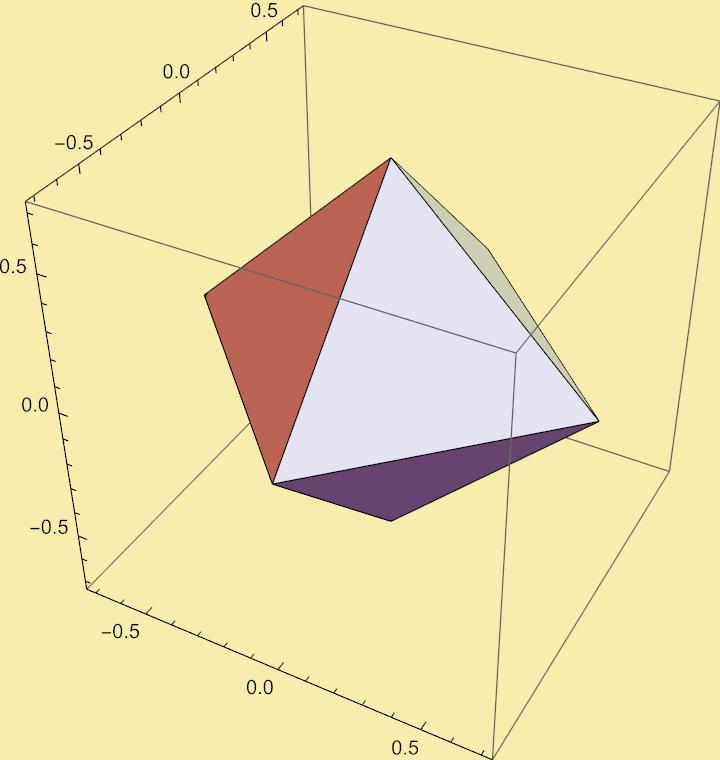
\includegraphics[width=\textwidth]{octahedron}
				\caption{Октаэдр}
				\label{fig:first}
			\end{subfigure}
			\hfill
			\begin{subfigure}{0.3\textwidth}
				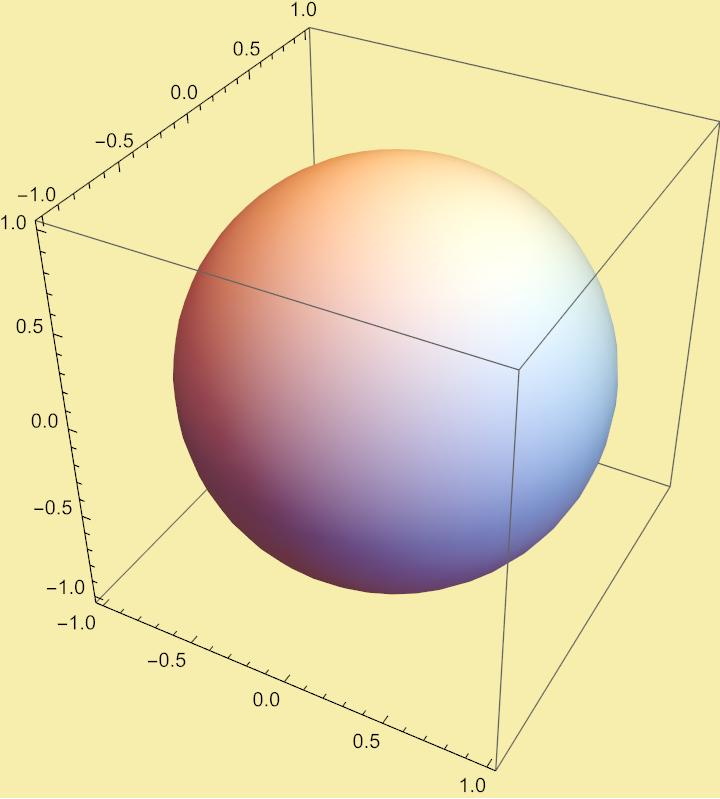
\includegraphics[width=\textwidth]{ball}
				\caption{Шар}
				\label{fig:second}
			\end{subfigure}
			\hfill
			\begin{subfigure}{0.3\textwidth}
				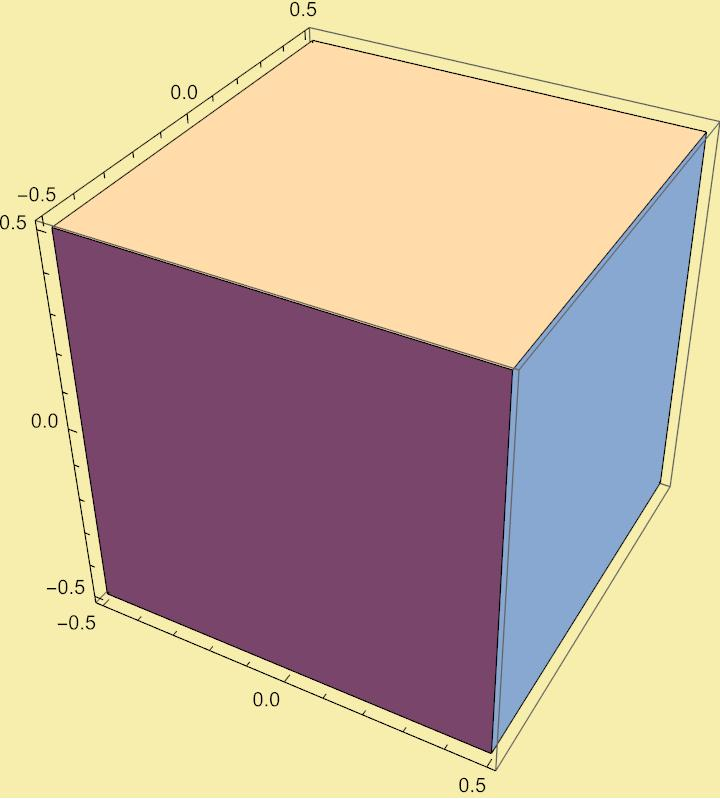
\includegraphics[width=\textwidth]{cube}
				\caption{Куб}
				\label{fig:third}
			\end{subfigure}
			
			\caption{Фигуры}
			\label{fig:figures}
		\end{figure}
	\end{enumerate}
	\newpage
	dcwds
	\newpage
\section{Результаты}

\footnotesize
\begin{center}
	\begin{tabular}{|c|c|}\hline
		%			\caption{Результаты теста №5}
		\multicolumn{2}{|c|}{Исходные данные: Тест №5}\\
		\hline \multicolumn{2}{|c|}{$A = $
			$
			\begin{pmatrix}
				28.859 & -0.008 & 2.406 & 19.240 \\ 
				14.436 & -0.001 & 1.203 & 9.624 \\ 
				120.204 & -0.032 & 10.024 & 80.144 \\ 
				-57.714 & 0.016 & -4.812 & -38.478 
			\end{pmatrix}
			$
			$,\qquad b = $
			$
			\begin{pmatrix}
				30.459 \\ 
				18.248 \\ 
				128.156 \\ 
				-60.908 
			\end{pmatrix}
			$
		} \\
		\hline
		обычная точность & повышенная точность \\
		\hline
		\multicolumn{2}{|c|}{Решение методом Гаусса} \\
		\hline
		$
		\begin{pmatrix}
			1.49898720 \\ 
			1000.24298096 \\ 
			-18.04016495 \\ 
			2.00656486 
		\end{pmatrix}
		$
		& 
		$
		\begin{pmatrix}
			0.9999999995029749 \\ 
			999.9999999997534132 \\ 
			-20.0000000019684592 \\ 
			3.0000000009915690 
		\end{pmatrix}
		$
		\\
		\hline \multicolumn{2}{|c|}{Норма вектора невязки $\|b - b_1 \|_1$}\\
		\hline
		1,526 $\cdot 10^{-5}$ & 1,07 $\cdot 10^{-14}$\\
		\hline \multicolumn{2}{|c|}{Норма вектора невязки $\|b - b_1 \|_2$}\\
		\hline
		1,206 $\cdot 10^{-5}$ & 0,79 $\cdot 10^{-14}$\\
		\hline \multicolumn{2}{|c|}{Норма вектора невязки 
			
			$\|b - b_1 \|_{\infty}$}\\
		\hline
		1,144 $\cdot 10^{-5}$ & 0,71 $\cdot 10^{-14}$\\
		\hline  \multicolumn{2}{|c|}{Погрешность метода Гаусса}\\
		\hline
		Что-то & написать \\
		\hline  \multicolumn{2}{|c|}{Решение методом QR-разложения}\\
		\hline
		$
		\begin{pmatrix}
			9.18884 \\ 
			2.22287 \\ 
			-1.23578 \\ 
			0.991991 
		\end{pmatrix}
		$
		& 
		$
		\begin{pmatrix}
			0.9999999982831136 \\ 
			999.9999999991688355 \\ 
			-20.0000000067030115 \\ 
			3.0000000034131191 
		\end{pmatrix}
		$
		\\
		\hline  \multicolumn{2}{|c|}{матрица Q}\\
		\hline
		\tiny{
			$
			\begin{pmatrix}
				0.21035759 & -0.10577760 & -0.50090319 & 0.83286071 \\ 
				0.10522618 & 0.97148943 & -0.21036340 & -0.02971083 \\ 
				0.87618512 & 0.01047287 & 0.47717786 & 0.06701660 \\ 
				-0.42068607 & 0.21191855 & 0.69075650 & 0.54860663 
			\end{pmatrix}
			$
			
		} & 
		
		\tiny{
			$
			\begin{pmatrix}
				0.21035761 & -0.1057774 & -0.50100780 & 0.83279768 \\ 
				0.1052261 & 0.97148953 & -0.21035973 & -0.02973746 \\ 
				0.87618511 & 0.01047290 & 0.47716945 & 0.06707656 \\ 
				-0.42068606 & 0.21191869& 0.69068753 & 0.54869338 
			\end{pmatrix}
			$
			
		}\\
		\hline \multicolumn{2}{|c|}{матрица R}\\
		\hline
		\tiny{
			$
			\begin{pmatrix}
				137.19018555 & -0.03655699 & 11.43992901& 91.46811676 \\ 
				0.00000087 & 0.00293030 & -0.00057107 & -0.00041090 \\ 
				0.00000003 & 0.00000000 &  0.00107075 & 0.00209990 \\ 
				-0.00000038 & 0.00000000 & 0.00000000 & -0.00000616 
			\end{pmatrix}
			$
			
		} & 
		\tiny{
			$
			\begin{pmatrix}
				137.19018692 & -0.03655698 & 11.43992847 & 91.46811570 \\ 
				0.00000000 & 0.00293029 & -0.00057107 & -0.00041057 \\ 
				0.00000000 & 0.00000000 & 0.00107070 & 0.00210197 \\ 
				-0.00000000 & 0.00000000 & 0.00000000 & -0.00000557 
			\end{pmatrix}
			$
			
		}\\
		\hline \multicolumn{2}{|c|}{Норма вектора невязки $\|b - b_1 \|_1$}\\
		\hline
		0,954 $\cdot 10^{-5}$ & 9,24 $\cdot 10^{-14}$\\
		\hline \multicolumn{2}{|c|}{Норма вектора невязки $\|b - b_1 \|_2$}\\
		\hline
		0,572 $\cdot 10^{-5}$ & 6,13 $\cdot 10^{-14}$\\
		\hline \multicolumn{2}{|c|}{Норма вектора невязки $\|b - b_1 \|_{\infty}$}\\
		\hline
		0,381 $\cdot 10^{-5}$ & 5,68 $\cdot 10^{-14}$\\
		\hline  \multicolumn{2}{|c|}{Погрешность метода QR-разложения}\\
		\hline
		Что-то & написать \\
		\hline 
		\multicolumn{2}{|c|}{ Число обусловленности ($p = 1 $), $M_A$}\\
		\hline
		\multicolumn{2}{|c|}{$25741978.73944124 \leqslant 122414849.8883399 \leqslant 	321014390.09659916$}\\
    	\hline \multicolumn{2}{|c|}{Число обусловленности ($p = \infty $), $M_A$}\\
    	\hline \multicolumn{2}{|c|}{$91163201.12185164 \leqslant 109686235.2039425\leqslant 298220694.33281744$}\\
    	\hline
    
    	
    \end{tabular}
\end{center}

\footnotesize
\begin{center}
	\begin{tabular}{|c|c|}\hline
		%			\caption{Результаты теста №5}
		\multicolumn{2}{|c|}{Исходные данные: Вариант 1}\\
		\hline \multicolumn{2}{|c|}{$A = $
			$
			\begin{pmatrix}
				16.382 &  -2.049 & -41.829 & 16.392 \\ 
				307.648 & -38.466 & -840.366 & 312.528 \\ 
				0.456 & -0.057 & -1.177 & 0.456 \\ 
				23.272 & -2.909 & -66.309 & 23.872 
			\end{pmatrix}
			$
			$,\qquad b = $
			$
			\begin{pmatrix}
				33.613 \\ 
				710.342 \\ 
				0.949 \\ 
				57.673 
			\end{pmatrix}
			$
		} \\
		\hline
		обычная точность & повышенная точность \\
		\hline
		\multicolumn{2}{|c|}{Решение методом Гаусса} \\
		\hline
		$
		\begin{pmatrix}
			-5.03971243 \\ 
			-5.47288799 \\ 
			-1.14634335 \\ 
			3.47786856 
		\end{pmatrix}
		$
		& 
		$
		\begin{pmatrix}
			1.9999999949416818 \\ 
			59.9999999529556547 \\ 
			-1.0000000001051392 \\ 
			4.9999999989063948 
		\end{pmatrix}
		$
		\\
		\hline \multicolumn{2}{|c|}{Норма вектора невязки $\|b - b_1 \|_1$}\\
		\hline
		6,485 $\cdot 10^{-5}$ & 28,5 $\cdot 10^{-14}$\\
		\hline \multicolumn{2}{|c|}{Норма вектора невязки $\|b - b_1 \|_2$}\\
		\hline
		6,115 $\cdot 10^{-5}$ & 23,18 $\cdot 10^{-14}$\\
		\hline \multicolumn{2}{|c|}{Норма вектора невязки 
			
			$\|b - b_1 \|_{\infty}$}\\
		\hline
		6,104 $\cdot 10^{-5}$ & 22,74 $\cdot 10^{-14}$\\
		\hline  \multicolumn{2}{|c|}{Погрешность метода Гаусса}\\
		\hline
		Что-то & написать \\
		\hline  \multicolumn{2}{|c|}{Решение методом QR-разложения}\\
		\hline
		$
		\begin{pmatrix}
			-3.63152623 \\ 
			7.62731504 \\ 
			-1.11702025 \\ 
			3.78289294 
		\end{pmatrix}
		$
		& 
		$
		\begin{pmatrix}
			2.0000000198214503 \\ 
			60.0000001843341622 \\ 
			-0.9999999995881664 \\ 
			 5.0000000042833257 
		\end{pmatrix}
		$
		\\
		\hline  \multicolumn{2}{|c|}{матрица Q}\\
		\hline
		\tiny{
			$
			\begin{pmatrix}
				0.05302272 & 0.99574733 & 0.00147591 & 0.07532319 \\ 
				-0.68938291 & -0.01808131 & 0.01418723 & 0.72403234 \\ 
				0.63956553 & -0.07996984 & 0.47688016 & 0.59761691 \\ 
				0.33599940 & -0.04201264 & -0.87885261 & 0.33609143 
			\end{pmatrix}
			$
			
		} & 
		
		\tiny{
			$
			\begin{pmatrix}
				0.05302272 & 0.99574737 & 0.00147591 & 0.07532320 \\ 
				-0.68919382 & -0.01810496 & 0.01419047 & 0.59806831 \\ 
				0.64034437 & -0.08004305 & 0.47525413 & 0.59806831 \\ 
				0.33490232 & -0.04186279& -0.87973289 & 0.33489996 
			\end{pmatrix}
			$
			
		}\\
		\hline \multicolumn{2}{|c|}{матрица R}\\
		\hline
		\tiny{
			$
			\begin{pmatrix}
				308.96188354 & -38.63026047 & -844.00646973& 313.86688232 \\ 
				0.00000087 & 0.00104253 & -3.99544239 & 0.33928907 \\ 
				0.00000003 & 0.00000000 &  0.26287937 &  -0.02528645 \\ 
				-0.00000038 & 0.00000000 & 0.00000000 & -0.00000655 
			\end{pmatrix}
			$
			
		} & 
		\tiny{
			$
			\begin{pmatrix}
				308.96190016 & -38.63026127 & -844.00646641 & 313.86687148 \\ 
				0.00000000 &  0.00104254 & -3.99538137 & 0.33928294 \\ 
				0.00000000 & 0.00000000 &  0.26380419 & -0.02536564 \\ 
				-0.00000000 & 0.00000000 & 0.00000000 & -0.00000141 
			\end{pmatrix}
			$
			
		}\\
		\hline \multicolumn{2}{|c|}{Норма вектора невязки $\|b - b_1 \|_1$}\\
		\hline
		26,774 $\cdot 10^{-5}$ & 36,52 $\cdot 10^{-14}$\\
		\hline \multicolumn{2}{|c|}{Норма вектора невязки $\|b - b_1 \|_2$}\\
		\hline
		24,492 $\cdot 10^{-5}$ & 34,14 $\cdot 10^{-14}$\\
		\hline \multicolumn{2}{|c|}{Норма вектора невязки $\|b - b_1 \|_{\infty}$}\\
		\hline
		24,414 $\cdot 10^{-5}$ & 34,11 $\cdot 10^{-14}$\\
		\hline  \multicolumn{2}{|c|}{Погрешность метода QR-разложения}\\
		\hline
		Что-то & написать \\
		\hline 
		\multicolumn{2}{|c|}{ Число обусловленности ($p = 1 $), $M_A$}\\
		\hline
		\multicolumn{2}{|c|}{$25741978.73944124 \leqslant 28865938619.82852 \leqslant 	91055029023.15531921$}\\
		\hline \multicolumn{2}{|c|}{Число обусловленности ($p = \infty $), $M_A$}\\
		\hline \multicolumn{2}{|c|}{$91163201.12185164 \leqslant 72709218159.2467\leqslant 142703407569.15933228$}\\
		\hline
		
		
	\end{tabular}
\end{center}







\newpage
\begin{thebibliography}{1}
	\bibitem{galanin} \textit{Галанин М.П., Савенков Е.Б.} Методы численного анализа математических\\ моделей. М.: Изд-во МГТУ им. Н.Э. Баумана,	2010. 592 с.
	
	
\end{thebibliography}


\end{document}
